\documentclass{beamer}
\usepackage[utf8]{inputenc}
\usepackage{parskip, graphicx, caption, hyperref, enumerate}
\usepackage{mathtools, mathrsfs, amsmath, amsthm, amssymb}
\usepackage{tikz, tikz-cd}
\usepackage{biblatex}
\usetheme{Antibes}
\usecolortheme{beaver}
\urlstyle{same}
\addbibresource{history_linalg.bib}
\setbeamertemplate{bibliography item}[triangle]

\newcommand{\C}{\mathbb{C}}
\newcommand{\R}{\mathbb{R}}
\newcommand{\Z}{\mathbb{Z}}
\newcommand{\N}{\mathbb{N}}
\DeclareMathOperator{\Mat}{Mat}
\DeclareMathOperator{\End}{End}
\DeclareMathOperator{\Hom}{Hom}
\DeclareMathOperator{\Id}{Id}
\DeclareMathOperator{\rank}{rank}
\DeclareMathOperator{\trace}{tr}
\DeclareMathOperator{\Spec}{Spec}
\DeclareMathOperator{\img}{img}
\newcommand{\norm}[1]{\left\lVert#1\right\rVert}
\newcommand{\transpose}{\intercal}

\makeatletter
\renewcommand*\env@matrix[1][*\c@MaxMatrixCols c]{%
  \hskip -\arraycolsep
  \let\@ifnextchar\new@ifnextchar
  \array{#1}}
\makeatother

\newenvironment{lbmatrix}[1]
  {\left[\array{@{}*{#1}{c}@{}}}
  {\endarray\right]}

\theoremstyle{definition}
\newtheorem*{definition*}{Definition}
\newtheorem*{theorem*}{Theorem}
\newtheorem*{proposition*}{Proposition}
\newtheorem*{problem*}{Problem}
\newtheorem*{example*}{Example}
\newtheorem*{remark*}{Remark}


\title{A History of Computational Linear Algebra}
\subtitle{The Theory of Tables of Numbers through Time}
\author{Jesse He}
\institute{OSU Reading Classics}
\date{16 February, 2020}

\begin{document}
    
\frame{\titlepage}

\section{Linear Systems and Gaussian Elimination}
\begin{frame}
    \frametitle{Sheaves of wheat}

    Systems of simultaneous linear equations are known to have been computed as far back as ancient Mesopotamia, but we will begin with the first matrices.
    \pause
    Consider the following problem:

    \begin{problem}
        ``The yield of 3 sheaves of superior grain, 2 sheaves of medium grain, and 1 sheaf of inferior grain is 39 pieces of bread.

        The yield of 2 sheaves of superior grain, 3 sheaves of medium grain, and 1 sheaf of inferior grain is 34 pieces of bread.

        The yield of 1 sheaf of superior grain, 2 sheaves of medium grain, and 3 sheaves of inferior grain is 26 pieces of bread.

        What is the yield of superior, inferior, and medium grains?''
    \end{problem}
\end{frame}

\begin{frame}
    \frametitle{Sheaves of wheat}

    With $x$ representing superior grain, $y$ representing medium grain, and $z$ representing inferior grain, we have a system of linear equations:
    \begin{alignat*}
        3x & + & 2y & + & z & = 39 \\
        2x & + & 3y & + & z & = 34 \\
        1x & + & 2y & + & 3z & = 26
    \end{alignat*}
    which we can solve with Gaussian elimination.

    However, the Chinese mathematicians who wrote this problem did not have the benefit of Gauss's work, since this was published in the
    \textit{Nine Chapters on the Art of Calculation} about 600 years before Gauss's birth.\cite{vdw}
\end{frame}

\begin{frame}
    \frametitle{Sheaves of wheat}

    To solve, we simply represent this as a matrix and perform Gaussian elimination the usual way:
    \pause
    \begin{center}
        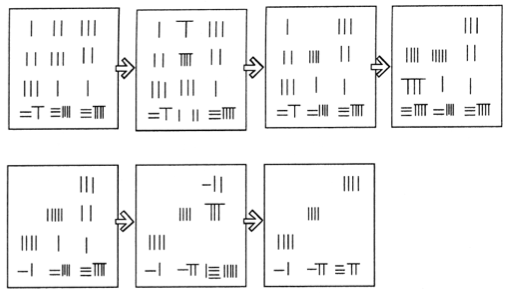
\includegraphics{Images/NineChaptersMatrix.png}
        \hspace*{15pt}\hbox{\scriptsize Adapted from Horng Wann-Sheng by Randy K. Schwartz \cite{maa}}
    \end{center}
\end{frame}

\begin{frame}
    \frametitle{Sheaves of wheat}
    In more familiar notation,
    {\scriptsize
        \begin{alignat*}{3}
            \begin{bmatrix}[ccc|c]
                3 & 2 & 1 & 39 \\
                2 & 3 & 1 & 34 \\
                1 & 2 & 3 & 26
            \end{bmatrix} &\rightarrow
            \begin{bmatrix}[ccc|c]
                3 & 2 & 1 & 39 \\
                0 & 5 & 1 & 26 \\
                1 & 2 & 3 & 26
            \end{bmatrix} &\rightarrow
            \begin{bmatrix}[ccc|c]
                3 & 2 & 1 & 39 \\
                0 & 5 & 1 & 26 \\
                0 & 4 & 8 & 39
            \end{bmatrix} &\rightarrow
            \begin{bmatrix}[ccc|c]
                3 & 2 & 1  & 39 \\
                0 & 5 & 1  & 26 \\
                0 & 0 & 36 & 99
            \end{bmatrix} \\
            &\rightarrow
            \begin{bmatrix}[ccc|c]
                3 & 2 & 1 & 39 \\
                0 & 5 & 1 & 26 \\
                0 & 0 & 4 & 11
            \end{bmatrix} &\rightarrow
            \begin{bmatrix}[ccc|c]
                12 & 8 & 0 & 145 \\
                0  & 4 & 0 & 17 \\
                0  & 0 & 4 & 11
            \end{bmatrix} &\rightarrow
            \begin{bmatrix}[ccc|c]
                4 & 0 & 0 & 37 \\
                0 & 4 & 0 & 17 \\
                0 & 0 & 4 & 11
            \end{bmatrix}
        \end{alignat*}
        }
    so $x = \frac{37}{4}$, $y = \frac{17}{4}$, $z = \frac{11}{4}$.
\end{frame}

\begin{frame}
    \frametitle{Gaussian elimination, 600 years before Gauss}

    The Chinese matrix (\textit{f\={a}ngch\v{e}ng}) method described in the \textit{Nine Chapters} was used to solve equations in several unknowns,
    including a procedure for handling negative numbers and an exercise with 6 unknowns in 5 equations.

    \pause
    The method appeared later in Newton's notes in 1670, and methods of elimination and matrix reduction were developed in Europe throughout the 18th and 19th centuries
    including Gauss's contribution in 1811\cite{roots}\cite{internet}.
\end{frame}

\begin{frame}
    \frametitle{Determinate and indeterminate systems}

    \begin{definition}
        A system of linear equations is said to be \underline{underspecified} if there are fewer equations than unknowns.

        If there are more equations than unknowns, the system is said to be \underline{overspecified}.
    \end{definition}
    \begin{definition}
        A system of equations is \underline{determinate} if there is a unique solution.
        If there is more than one solution, it is \underline{indeterminate}.
    \end{definition}
\end{frame}

\begin{frame}
    \frametitle{Determinate and indeterminate systems}

    \begin{remark*}
        An underspecified linear system must necessarily be indeterminate, but the converse may not hold.
    \end{remark*}
    \pause
    Under what conditions is a linear system of equations determinate?
\end{frame}

\section{The Determinant}

\begin{frame}
    \frametitle{Discovery}
    
    The determinant of a matrix was used as a tool for solving simultaneous polynomial equations by Japanese mathematician Seki K\={o}wa in 1683\cite{japan-det},
    and introduced independently by Leibnitz in 1693\cite{hist-alg}
    
    \pause
    Seki illustrates the $2\times 2$ case with the following picture:

    \begin{center}
        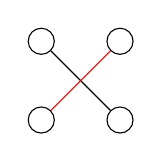
\begin{tikzpicture}
            \node[circle, draw] at (0, 0) (a) {};
            \node[circle, draw] at (1, 0) (b) {};
            \node[circle, draw] at (0, -1) (c) {};
            \node[circle, draw] at (1, -1) (d) {};

            \draw[black] (a) -- (d);
            \draw[red] (b) -- (c);
        \end{tikzpicture}
    \end{center}

    where the red line corresponds to a positive (``constructive'') product and the black to a negative (``destructive'') product.
\end{frame}

\begin{frame}
    \frametitle{Laplace exapansion, half a century before Laplace}

    Seki describes the method for calculating determinants up to the $5\times 5$ case in his \textit{Fukudai} in 1683, and by 1710 Seki and his contemporaries
    had described a full, correct description of the Laplace expansion.

    \pause
    In Europe, Gabriel Cramer used the determinant in 1750 to describe closed-form solutions to systems of linear equations in terms of their coefficients
    (what we now call \underline{Cramer's rule}), and other European mathematicians would continue to study determinants throughout the 18th and 19th centuries.
\end{frame}

\begin{frame}
    \frametitle{Singular and nonsingular matrices}
    
    Cramer noted that system whose determinant was zero did not have a unique solution, and moreover used his closed-form solutions to characterize when
    a system had zero, one, or infinitely many solutions.

    Euler noticed in the same year that a system of $n$ equations in $n$ unknowns need not have a unique solution:
    \begin{align*}
        3x-2y &= 5 \\
        6x-4y &= 10
    \end{align*}
    which led to the idea of ``inclusive dependence'' (what we now refer to as \textit{linear dependence})\cite{roots}.
\end{frame}

\section{Vector Spaces}

\begin{frame}
    \frametitle{Algebra with tables of numbers}

    James Joseph Sylvester coined the term ``matrix'' in 1850, and his collegue Arthur Cayley published his \textit{Treatise on the Theory of Matrices}
    where he developed a theory of matrix addition, multiplication, and inversion.

    \pause
    Let $\mathbb{F}$ be a field. For now, a matrix is a table of numbers, which we write $A = (a_{ij})$; $a_{ij}$ is the entry in the $i$-th row and $j$-th column
    of $A$.

    \pause
    Given two $n \times m$ matrices $A = (a_{ij})$ and $B = (b_{ij})$, we write their sum $A + B = (a_{ij} + b_{ij})$.

    \pause
    Given an $n \times m$ matrix $A$ and an $m \times n$ matrix $B$, we write their product $AB = \left( \sum_{k=1}^n a_{ik} b_{kj} \right)$.

    \pause
    Given a matrix $A$ and a scalar $\lambda$, the scalar product is $\lambda A = (\lambda a_{ij})$.
\end{frame}

\begin{frame}
    \frametitle{Algebra with tables of numbers}

    The $n \times n$ identity matrix is the matrix
    \[
        I = \begin{pmatrix}
            1 & 0 & \ldots & 0 \\
            0 & 1 & \ldots & 0 \\
            \vdots & \vdots & \ddots & \vdots \\
            0 & 0 & \ldots & 1
        \end{pmatrix}  
    \]
    with the property that $AI = IA = A$ for any matrix $A$ (where $I$ is understood to be of the proper size).

    The inverse $A^{-1}$ of an $n \times n$ matrix $A$ is the matrix such that $A A^{-1} = A^{-1} = A$.
\end{frame}

\begin{frame}
    \frametitle{Abstract lists of numbers}
    Frobenius identified a linear equation in $n$ variables with its $n$-tuple of coefficients, and formulated a definition of linear dependence that
    applied to both linear equations and $n$-tuples.

    \pause
    Hamilton used the term ``vector'' (which he borrowed from physics) to describe the non-real parts of his quaternions.

    \pause
    Weierstrass and Kronecker treated the determinant rigorously around 1860 (as a ``normed, linear, homogeneous function'')\cite{hist-alg}.

    \pause
    For completeness's sake, I will include some basic definitions and results from linear algebra.
\end{frame}

\begin{frame}
    \frametitle{Vectors}
    
    Peano gave a formal definition of a vector space in 1880\cite{hist-alg}.
    \pause
    \begin{definition}
        A vector space over a field $\mathbb{F}$ is a set $V$ with operations addition $+: V \times V \longrightarrow V$ and scalar
        multiplication $\bullet : \mathbb{F} \times V \longrightarrow V$ such that
        \begin{itemize}
            \item For all $u, v, w \in V$, $u + (v + w) = (u + v) + w$
            \item For all $u, v \in V$, $u + v = v + u$
            \item There exists $0_V \in V$ such that for all $v \in V$, $v + 0_V = v$
            \item For all $v \in V$, there exists $-v \in V$ so $v + (-v) = 0_V$
            \item For all $\lambda, \mu \in \mathbb{F}$, $v \in V$, $\lambda(\mu v) = (\lambda \mu)v$
            \item For all $v \in V$, $1_\mathbb{F} v = v$
            \item For all $\lambda \in \mathbb{F}$, $u, v \in V$, $\lambda(u+v) = \lambda u + \lambda v$
            \item For all $\lambda, \mu \in \mathbb{F}$, $v \in V$, $(\lambda + \mu)v = \lambda v + \mu v$
        \end{itemize}
    \end{definition}
\end{frame}

\begin{frame}
    \frametitle{Vectors}

    \begin{definition}
        A set $U \subseteq V$ is a linear subspace of $V$ if $U$ is a vector space under the operations on $V$.
    \end{definition}
    \begin{proposition*}
        $U \subseteq V$ is a linear subspace of $V$ if and only if $U$ is closed under vector addition and scalar multiplication.
    \end{proposition*}
\end{frame}

\begin{frame}
    \frametitle{Linear combinations}
    \begin{definition}
        A linear combination of a set $S \subseteq V$ is a finite sum
        \[
            \sum_{v \in S} \alpha_v v
        \]
        where $\alpha_v \in \mathbb{F}$ and only finitely many are nonzero.

        The set of all linear combinations of $S$ is the span of $S$.
    \end{definition}
\end{frame}

\begin{frame}
    \frametitle{Linear dependence and independence}

    \begin{definition}
        A set $S \subseteq V$ is linearly dependent if there exist $(\alpha_v)_{v \in V}$, finitely many nonzero, not all zero, such that
        \[
            0 = \sum_{v \in S} \alpha_v v
        \]
        If $S$ is not linearly dependent we say it is linearly independent.
    \end{definition}
\end{frame}

\begin{frame}
    \frametitle{Basis and dimension}

    \begin{definition}
        A basis for a vector space $V$ is a maximal linearly independent set $S \subseteq V$.

        Equivalently, $S$ is linearly independent and $\operatorname{span}(S) = V$.
    \end{definition}
    \begin{definition}
        The dimension of $V$ is the cardinality of a basis for $V$.
    \end{definition}
\end{frame}

\begin{frame}
    \frametitle{Tables of numbers acting on lists of numbers}

    From this new perspective of vector spaces, the theory of matrices was recontextualized as the theory of linear maps between vector spaces.
    \pause
    \begin{definition}
        A function $T: V \longrightarrow W$ between vector spaces is linear if for all $u, v \in V$, $\lambda, \mu \in \mathbb{F}$,
        \[
            T(\lambda v + \mu u) = \lambda T(v) + \mu T(u).
        \]
    \end{definition}
    Frequently we write $Tv$ to mean $T(v)$.
    \pause
    A linear map can be encoded as a matrix by choosing a basis for $V$ and then writing the images of each basis vector in terms of the basis.
\end{frame}

\begin{frame}
    \frametitle{Kernels and images}

    \begin{definition}
        Let $U, V$ be vector spaces and let $T: V \longrightarrow W$ be a linear map. Then
        \[
            \ker(T) = \{v \in V \mid Tv = 0_W\}, \ \img(T) = \{Tv | v \in V\}.
        \]
    \end{definition}
    \begin{proposition*}
        $\ker(M)$ and $\img(M)$ are linear subspaces.
    \end{proposition*}
\end{frame}

\section{Eigenvalues and Spectral Theory}

\begin{frame}
    \frametitle{The characteristic polynomial}

    Cayley's work defining matrix operations, as well as the identity matrix $I$, allowed for a more algebraic treatment of matrices.

    \pause
    \begin{definition}
        The characteristic polynomial of a square matrix $M$ is $p(\lambda) = \det(M - \lambda I)$
    \end{definition}

    \pause
    Cayley gave a proof of the Cayley-Hamilton theorem in 1858 (Frobenius gave a full proof in 1878):
    \begin{theorem*}[Cayley-Hamilton, 1858]
        Any square matrix $M$ satisfies its characteristic polynomial.
    \end{theorem*}
\end{frame}

\begin{frame}
    \frametitle{Eigenvalues, eigenvectors, and eigenspaces}

    Euler first observed ``principal axes'' when studying rotational motion, which Lagrange later noticed were eigenvectors:
    \pause
    \begin{definition}
        Let $T: V \longrightarrow V$ be a linear map. We say $\lambda \in \mathbb{F}$ is an eigenvalue of $T$ if there is some $v \in V$, $v \neq 0_V$ such that
        \[
            Tv = \lambda v.
        \]
        The vector $v$ is said to be an eigenvector of $T$ associated with $\lambda$, and the set of all such vectors is called the eigenspace associated with $\lambda$.
    \end{definition}
    Cauchy coined the term ``characteristic root'' for the idea of eigenvalues.
\end{frame}

\begin{frame}
    \frametitle{Eigenvalues and the characteristic polynomial}
    \begin{proposition*}
        Consider a matrix $M$ as a linear transformation $M: V \longrightarrow V$. Then the eigenvalues of $M$ are the roots of its characteristic polynomial.
    \end{proposition*}
    \pause
    \begin{definition}
        The set of eigenvalues of $M$ is the spectrum of $M$, $\Spec(M)$. For convenience, allow $\Spec(M)$ to have multiple copies of the same element,
        accounting for multiplicity. 
    \end{definition}
    \pause
    \begin{proposition*}
        \[\det(M) = \prod_{\lambda \in \Spec(M)} \lambda\]
    \end{proposition*}
\end{frame}

\begin{frame}
    \frametitle{Eigenvalue algorithms}

    There are a number of algorithms to find the spectrum of a matrix:

    \pause
    The naive algorithm is to simply expand the characteristic polynomial $p(\lambda) = \det(T - \lambda I)$ and solve for $\lambda$.

    \pause
    Some algorithms are iterative, producing a sequence of values that converges to an eigenvalue, like Jacobi's algorithm, power iteration, or the QR algorithm.

    \pause
    Others involve direct calculation, but there are no general (non-naive) algorithms to directly calculate the spectrum of an arbitrary matrix.
\end{frame}

\begin{frame}
    \frametitle{Generalized eigenspaces}

    \begin{definition}
        Let $V$ be a vector space, let $T: V \longrightarrow V$ be a linear map, and let $\lambda$ be an eigenvalue of $T$.
        The generalized eigenspace associated with $\lambda$ is the subspace $E_\lambda = \{v \in V \mid (T - \lambda I)^n v = 0_V \text{ for some } n \in \N\}$.
    \end{definition}
    \begin{theorem*}[Jordan Decomposition, 1870]
        If $V$ is finite-dimensional and $T: V \longrightarrow V$ has all its eigenvalues in $\mathbb{F}$, (i.e. its characteristic polynomial splits), then
        we can decompose $V$ into its generalized eigenspaces
        \[
            V = \bigoplus_{\lambda \in \Spec(T)} E_\lambda  
        \]
    \end{theorem*}
\end{frame}

\begin{frame}
    \frametitle{Jordan canonical form}
    The Jordan canonical form expresses the spectrum and generalized eigenspaces of a transformation:
    \[
        \operatorname{JCF}(T) = \begin{pmatrix}
            J_0 & 0 & \ldots & 0 \\
            0 & J_1 & \ldots & 0 \\
            \vdots & \vdots & \ddots & \vdots \\
            0 & 0 & \ldots & J_n
        \end{pmatrix}
    \]
    where $\Spec(T) = \{\lambda_0, \ldots, \lambda_n\}$ and each Jordan block $J_i$ is of the form
    \[
        J_i = \begin{pmatrix}
            \lambda_i & 1 & 0 & \ldots & 0 \\
            0 & \lambda_i & 1 & \ldots & 0 \\
            \vdots & \vdots & \vdots & \ddots & \vdots \\
            0 & 0 & 0 & \ldots & \lambda_i
        \end{pmatrix}
    \]
\end{frame}

\begin{frame}
    \frametitle{Finding Jordan normal form}

    The algorithm to find the Jordan normal form of a linear transformation $T$ (assuming the characteristic polynomial splits) is, at a high level, as follows:

    \pause
    Calculate $\Spec(T)$.

    \pause
    For each $\lambda \in \Spec(T)$, calculate the associated generalized eigenspace $E_\lambda$.

    \pause
    Start with a basis for $E_\lambda$ and iteratively find a Jordan basis for $E_\lambda$.

    \pause
    Gather all the Jordan bases for each $E_\lambda$ into a Jordan basis for $T$.
\end{frame}

\begin{frame}
    \frametitle{The $J_0 \ker(S)$ trick}
    
    Computing the Jordan canonical form of a linear map can be computationally expensive, and the Jordan canonical form is very sensitive
    to small numerical changes.

    \pause
    To verify that the result of such a computation is correct, we can test each Jordan block, beginning with $J_0$:

    \pause
    Let $S = T - \lambda_0 I$. Then $E_{\lambda_0} = \ker(S^{n-1})$, so we apply the restriction of $T_{E_{\lambda_0}} = J_0$ to the kernel of $S$
    to verify that
    \[
        J_0 \ker(S) = (J_0)^2 \ker(S^2) = \cdots = (J_0)^n \ker(S^n) = \{0_V\}
    \]
    and then we can repeat this ``$J_0 \ker(S)$ trick'' for each Jordan block.
\end{frame}

\begin{frame}
    \title{References}
    \printbibliography
\end{frame}

\end{document}